\documentclass[DIV15, a4paper]{article}

% --------------------------------------------------------------------
% Define our own paper format
% --------------------------------------------------------------------
\setlength\textwidth{6.5in}
\setlength\textheight{9.5in}
\setlength\oddsidemargin{-0.25in}
\setlength\topmargin{-0.25in}
\setlength\headheight{0in}
\setlength\headsep{0in}
\setlength\columnsep{18pt}
\sloppy

% --------------------------------------------------------------------
% Packages
% --------------------------------------------------------------------
\usepackage[ruled, linesnumbered, vlined, commentsnumbered]{algorithm2e}
\usepackage{authblk}
\usepackage{prettyref}
\usepackage{graphicx}
\usepackage{diagbox}
\usepackage{booktabs}
\usepackage{colortbl}
\usepackage{amssymb}
\usepackage{amsfonts}
\usepackage{amsmath}
\usepackage{amsthm}
\usepackage{multirow}
\usepackage{tabularx}
\usepackage{footnote}
\usepackage{threeparttable}
\usepackage{hyperref}
\usepackage{amsopn}
\usepackage{cite}
\usepackage{setspace}
\usepackage{hhline}
\usepackage{color}
\usepackage{xcolor}  % Required for custom colors
\usepackage{rotating}

\usepackage{verbatim}
\usepackage{subcaption}

% Colors
% Define a few colors for making text stand out within the presentation
\definecolor{myblue}{RGB}{34,31,217}

\definecolor{mycyan}{gray}{.7}
\newtheorem{remark}{Remark}
\newtheorem{theorem}{Theorem}
\newtheorem{proposition}{Proposition}
\newtheorem{corollary}{Corollary}
\newtheorem{definition}{Definition}
\newtheorem{lemma}{Lemma}
\newtheorem{property}{Property}

\DeclareMathOperator*{\argmax}{argmax}
\DeclareMathOperator*{\argmin}{argmin}

% correct bad hyphenation here
\hyphenation{op-tical net-works semi-conduc-tor}

\newcommand{\bb}[1]{\multicolumn{1}{>{\columncolor{mycyan}}c}{\textbf{{#1}}}}
\newcommand\notealf[1]{\mbox{}\marginpar{\footnotesize\raggedright\hspace{0pt}\color{blue}\emph{#1}}}
\newcommand{\pref}{\prettyref}
\newcommand{\STAB}[1]{\begin{tabular}{@{}c@{}}#1\end{tabular}}

\newrefformat{fig}{Figure~\ref{#1}}
\newrefformat{tab}{Table~\ref{#1}}
\newrefformat{sec}{Section~\ref{#1}}
\newrefformat{app}{Appendix~\ref{#1}}
\newrefformat{alg}{Algorithm~\ref{#1}}
\newrefformat{property}{Property~\ref{#1}}
\newrefformat{theorem}{Theorem~\ref{#1}}
\newrefformat{corollary}{Corollary~\ref{#1}}
\newrefformat{proposition}{Proposition~\ref{#1}}
\newrefformat{def}{Definition~\ref{#1}}
\newrefformat{eq}{equation~(\ref{#1})}

\renewcommand\qedsymbol{$\blacksquare$}

\usepackage{graphicx}
\definecolor{Gray}{gray}{0.9}
\usepackage{scrpage2}

%\usepackage{datetime}

%\pagestyle{scrheadings}
%\ohead{D2.7 -- How to Design Self-aware Systems}
%\ihead{FP7-257906 EPiCS}
%\cfoot{Page \thepage\ of \pageref{LastPage}}

\usepackage{lscape}

\newcommand\setItemnumber[1]{\setcounter{enumi}{\numexpr#1-1\relax}}
\newcommand*{\email}[1]{%
    \normalsize\href{mailto:#1}{#1}\par
    }

\begin{document}

\noindent Re: No. \textit{CYB-E-2021-05-1216}\\
{\textbf{TITLE:}}\ \textbf{Multi-Objective Virtual Network Function Placement: A Formal Model and Effective Algorithms}\\

\noindent Dear Editor-in-Chief,\\

We would like to thank you, the associate editor and the anonymous reviewers for their constructive comments on our manuscript. Following your suggestions, we have carefully revised our manuscript. Please find our point-by-point responses and the revised manuscript in this document.\\\\

Yours Sincerely,\\\\
Joseph Billingsley, Ke Li, Wang Miao, Geyong Min, Nektarios Georgalas
\clearpage

% !TeX root = main.tex

\noindent\textbf{--\ Response to Associate Editor}\\

\textsf{Authors are suggested to think which area they aim to contribute, a network communication area or an evolutionary computation area, revise this manuscript and choose a journal in the best area. If they aim to contribute in an EC area, our transactions is a good choice but emphasize their contribution to the EC research; if not, consider the suggestion of the second referee.}\\
\textcolor{blue}{\textbf{\textit{Reply}: We thank the associate editor for their comments. It is our goal with this work to introduce an important problem to the EC community, one which we believe that EC is well positioned to solve. By way of illustration, we developed new models and operators to demonstrate how EC concepts can improve the state of the art in this area. In the updated manuscript, we have made several modifications to emphasize our contributions to EC and \textit{vice versa}, EC research to the VNFPP. In particular, we would like to bring the attention of the associated editors to the following changes that are particularly pertinent:
        \begin{enumerate}
            \item To make clear the particular relevance of this research to Transactions on Cybernetics, we have updated many of the references to refer to relevant papers previously published in this journal.
            \item We have also extended the experiments section to have a greater focus on the evolutionary algorithm at the core of the paper. In particular we have conducted further experiments to analyse different solution representations in detail (see response to reviewer 1, points 3 and 5), and of different evolutionary frameworks (see response to review 3, point 2).
        \end{enumerate}}}

\textsf{This manuscript was submitted in this May, and authors' paper with a similar title was presented at EMO2021 held in this March. Please answer to the question from the third referee; it may be better to provide the EMO2021 paper together with authors' answer to three referees for fair check if authors submit their revision.
}\\
\textcolor{blue}{\textbf{\textit{Reply}: We have prepared a detailed response to this question in answer to the comments of the third referee.}}

\clearpage


% !TeX root = main.tex

\noindent\textbf{--\ Response to Reviewer $\sharp1$}\\

\textsf{To minimize the environmental impact of data centers, it is imperative to make data centers more energy efficient while maintaining a high quality of service (QoS). For evaluating the QoS of a data center, an analytical model using queueing theory is proposed. Based on this model, a domain-specific evolutionary optimization framework is developed for finding the optimal placement of virtual network functions in a data center that optimizes multiple conflicting objectives with regard to energy consumption and QoS.}

\textsf{There are some comments about this paper as follows.}

\begin{enumerate}
      \item \textsf{Is the relationship of the five constraints mutually independent or coupling?}\\
            \textcolor{blue}{\textbf{\textit{Reply}: We thank the reviewer for this suggestion. In the updated manuscript we elaborate further on the effect that these constraints have on the difficulty of the problem.}}\\
            \textcolor{blue}{\textit{``The combination of the constraints and objectives results in a challenging optimization problem. Although each of the constraints can be considered independently, each constraint is complex such that the feasible search space is small relative to the overall search space. Further, the NP-Hardness of the problem means that the feasible search space still contains many solutions, few of which will be at or near optimal."} \textbf{(Page x, highlighted in \textcolor{red}{red} color.)}}\\

      \item\textsf{Why do the authors design two tailored features in terms of a solution representation and an initialization operator? Not other tailored features? Please give reasons.}\\
            \textcolor{blue}{\textbf{\textit{Reply}: We thank the reviewer for this suggestion. In the process of our research we explored several alternative mutation and crossover operators but did not find any operators that led to significant improvements. Given the length of the manuscript currently, we did not consider these null results significant enough to include. In light of this comment, we have included some further explanation in the updated manuscript.}}\\
            \textcolor{blue}{\textit{``Further, we found the classic uniform crossover and mutation reproduction operators to be sufficient to vary and exchange information on the number and position of service instances."} \textbf{(Page x, highlighted in \textcolor{red}{red} color.)}}\\

      \item\textsf{Did you try other kinds of solution representations? Is it a genotype-phenotype solution representation suitable for the problem? Why?}\\
            \setItemnumber{5}
            \vspace{-2em}
      \item\textsf{Could you give the specific reasons why the binary and direct solution representations are only able to obtain feasible solutions to small data centers? And why can the proposed solution representation work? What is the essential difference?}\\
            \textcolor{blue}{\textbf{\textit{Reply}: We address comments 3 and 5 together. In the updated manuscript we have moved the comparison of different solution representations to a dedicated subsection with additional analysis.}}\\
            \textcolor{blue}{\textit{
                        ``To answer RQ3, we compare the quality of solutions obtained when different solution representations are applied to the VNFPP. Specifically, the following two meta-heuristic algorithms use NSGA-II as the baseline but have different solution representations.
                        \begin{itemize}
                              \item\underline{Binary representation}: As in [TODO], [TODO], [TODO], a string of binary digits are used to represent if a VNF is assigned to a server.
                              \item\underline{Direct representation}: As in [TODO], a solution is directly represented as a string of VNFs.
                        \end{itemize}
                        In our experiments, we generate $30$ VNFPP instances for six data centers with different sizes. To compare the performance of different algorithms, we use the QoS model developed in Section IV to evaluate the objective functions of the solutions obtained by different algorithms and use the HV indicator as the performance measure."
                  }}
            \begin{figure}[t!]
                  \centering
                  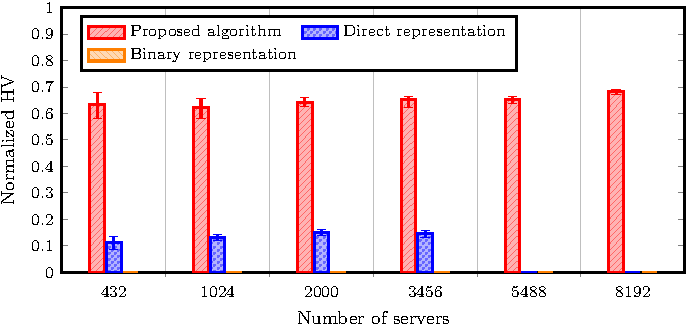
\includegraphics[width=.75\linewidth]{figs/comparison-crop}
                  \caption{The lower quartile, median, and upper quartile of the hyper-volume of the population for different algorithms on 30 VNFPP instances found by NSGA-II using different solution representations on 30 VNFPP instances}
            \end{figure}
            \begin{figure}[t!]
                  \centering
                  \begin{subfigure}[b]{0.3625\linewidth}
                        \includegraphics[width=\textwidth]{figs/qm-crop}
                        \caption{Proposed algorithm}
                  \end{subfigure}
                  \begin{subfigure}[b]{0.3625\linewidth}
                        \includegraphics[width=\textwidth]{figs/std-crop}
                        \caption{Direct representation}
                  \end{subfigure}

                  \vspace{1em}
                  \caption{An illustrative example of the final populations found by NSGA-II using our proposed representation and the direct solution representation. The binary solution representation is omitted as it resulted in no feasible solution at all.}
                  \label{fig:solution_representation_objectives}
            \end{figure}

            \textcolor{blue}{\textit{
                        ``From the results shown in Figs.~\ref{fig:solution_representation_comparison} and~\ref{fig:solution_representation_objectives}, we find that the solutions obtained by our proposed solution representation significantly outperform alternative representations. Our proposed solution representation has two advantages over existing representations. First, our proposed representation guarantees feasible solutions irregardless of the input. In contrast, both the direct and binary solution representations were unable to find feasible solutions to larger problem instances. Second, our proposed representation integrates domain knowledge to generate solutions with shorter average distances between VNFs causing the resultant solutions to be closer to the Pareto front than alternative representations. Existing solution representations do not utilize this information and instead rely solely on the optimization framework to locate high quality solutions.\\
                        Although the binary solution representation has been successfully applied to solve the VNFPP on small data centers (e.g.,~\cite{ChantreF20,KaurGK020,CharismiadisTPM20}), it does not scale well in the larger-scale problems considered in our experiments. With a binary solution representation, multiple VNFs to be placed on the same VM. This greatly complicates the search process compared to the direct or proposed solution representations with which this constraint is impossible to violate.\\
                        The direct solution representation is also only able to obtain feasible solutions to small data centers, as shown in~\pref{fig:alg_objectives}, and exclusively finds solutions with high energy consumption. In particular, since a solution is only feasible when there is an instance of each VNF, solutions with more VNFs are more likely to be feasible than those with less VNFs and lower energy consumption. This leads the algorithm with the direct representation to be biased towards solutions with a high energy consumption. On larger problems with high numbers of VNFs, the direct solution representation is unable to find a solution with at least one instance of each VNF."
                  } \textbf{(Page x, highlighted in \textcolor{red}{red} color.)}}\\
            \setItemnumber{4}

      \item\textsf{Section VI.B, p.9, “we apply our initialization operator to generate 100 randomly generated candidate solutions for each problem.”?}\\
            \textcolor{blue}{\textbf{\textit{Reply}: We apologize for the lack of clarity in this sentence. In the updated manuscript, this sentence reads as follows.}}\\
            \textcolor{blue}{\textit{``To create the benchmark, we generate 100 VNFPP problems for a data center with 412 servers to constitute a diverse set of
                        problems. Then, we use our proposed initialization operator (see Section V-B) to generate 100 candidate solutions for each problem."} \textbf{(Page x, highlighted in \textcolor{red}{red} color.)}}\\

            \setItemnumber{6}
      \item\textsf{Which key components of the proposed tailored EMO algorithm play roles to obtain solutions in terms of both convergence and diversity? Please give more discussions and analyses.}\\
            \textcolor{blue}{\textbf{\textit{Reply}: We thank the reviewer for this suggestion. In the updated manuscript, we elaborate further on the contributions of each of our tailored operators.}}
            \begin{figure*}[t!]
                  \centering
                  \begin{subfigure}[b]{0.32\linewidth}
                        \includegraphics[width=\textwidth]{figs/comparison/qm-crop}
                        \caption{Proposed algorithm}
                  \end{subfigure}
                  \begin{subfigure}[b]{0.32\linewidth}
                        \includegraphics[width=\textwidth]{figs/comparison/std-crop}
                        \caption{Direct representation}
                  \end{subfigure}

                  \vspace{1em}

                  \begin{subfigure}[b]{0.32\linewidth}
                        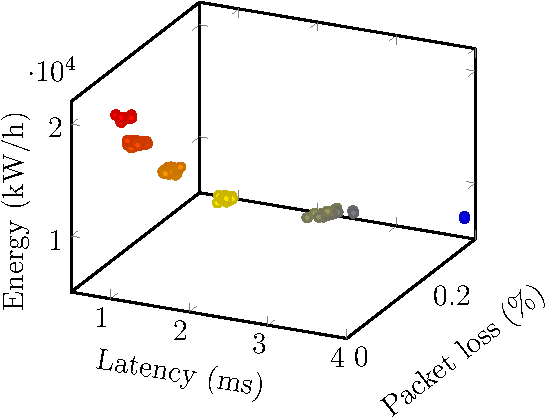
\includegraphics[width=\textwidth]{figs/comparison/esp_vdce-crop}
                        \caption{ESP-VDCE \cite{TODO}}
                  \end{subfigure}
                  \begin{subfigure}[b]{0.32\linewidth}
                        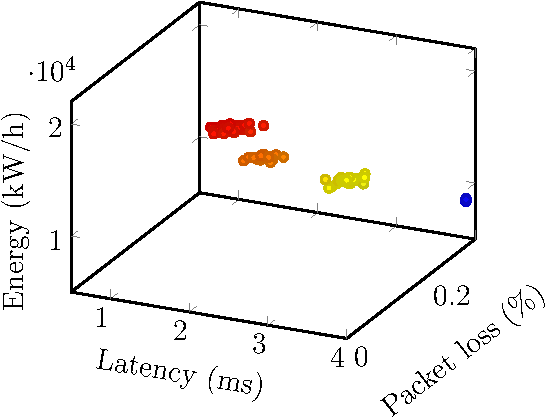
\includegraphics[width=\textwidth]{figs/comparison/bfdsu-crop}
                        \caption{BFDSU \cite{TODO}}
                  \end{subfigure}
                  \begin{subfigure}[b]{0.32\linewidth}
                        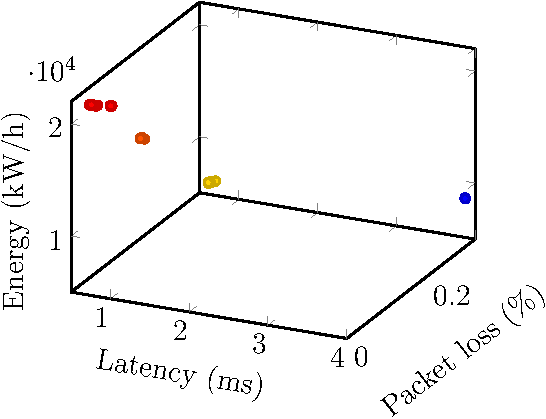
\includegraphics[width=\textwidth]{figs/comparison/stringer-crop}
                        \caption{Stringer \cite{TODO}}
                  \end{subfigure}

                  \vspace{1em}
                  \caption{An illustrative example of the objective values of the solutions in the final populations found by NSGA-II using our proposed algorithm and algorithms from the literature. Subproblems for the heuristic were generated using our proposed initialization operator. The binary solution representation is omitted as it resulted in no feasible solution at all.}
                  \label{fig:alg_objectives}
            \end{figure*}
            \begin{figure*}
                  \centering
                  \hfill
                  \begin{minipage}[t]{.48\textwidth}
                        \centering
                        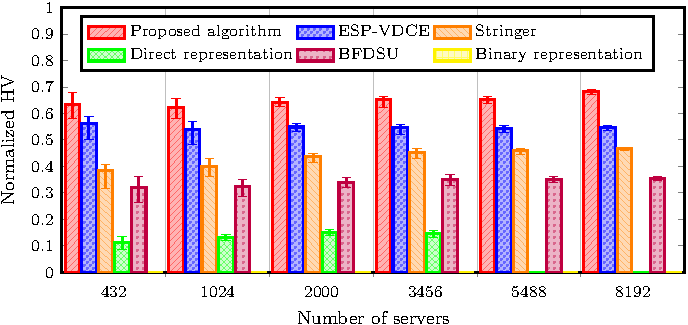
\includegraphics[width=\columnwidth]{figs/comparison/comparison-crop}
                        \caption{The lower quartile, median, and upper quartile of the hyper-volume of the population for different algorithms on 30 VNFPP instances using the initialization operator to generate subproblems for the heuristics.}
                        \label{fig:alg_comparison}
                  \end{minipage}\hfill
                  \begin{minipage}[t]{.48\textwidth}
                        \centering
                        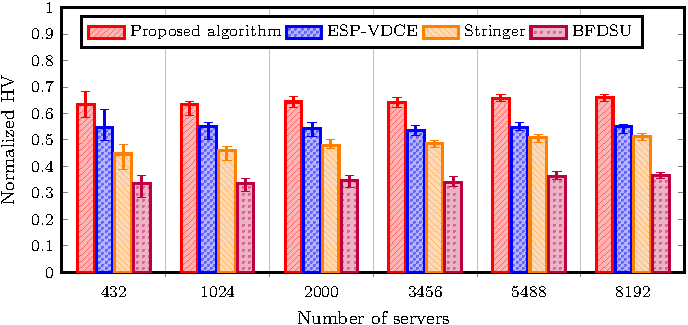
\includegraphics[width=\columnwidth]{figs/comparison/alg_fixed-crop}
                        \caption{The lower quartile, median, and upper quartile of the hyper-volume of the population for different algorithms on 30 VNFPP instances using the solutions of our proposed algorithm to generate subproblems for the heuristics.}
                        \label{fig:alg_fixed}
                  \end{minipage}
                  \hfill
            \end{figure*}\\
            \textcolor{blue}{\textit{
                        ``From the results shown in~\pref{fig:alg_comparison} and~\pref{fig:alg_fixed}, it is clear that our proposed algorithm outperforms other competitors on all test cases. This can be attributed to our two proposed operators. First, it is clear from \pref{fig:alg_objectives} that proposed operators enable a diverse population of solutions. Our two proposed operators work together towards this goal. The initialization operator produces a diverse range of possible solutions, whilst the solution representation ensures that these solutions are feasible.\\
                        Second, our proposed solution representation minimizes the distance between sequential VNFs, improving the overall QoS. We note that the two best performing algorithms, our proposed algorithm and ESP-VDCE, aim to minimize the distance between sequential VNFs. In contrast, both BFDSU and Stringer tend to produce longer path lengths thus lead to significantly worse solutions than our proposed algorithm. Since Stringer restricts the capacity of each server, it causes services to be placed across multiple servers. Likewise, the stochastic component of BFDSU can cause it to place VNFs far away from any other VNF of the service. In contrast, our proposed algorithm incorporates useful information into the optimization process and places sequential VNFs close by thus leading to better solutions.\\
                        A final benefit of our algorithm is that it can iteratively improve the placements to minimize the energy consumption and QoS. Although ESP-VDCE does consider the path length, it otherwise uses a simple first fit heuristic that cannot consider how service instances should be placed in relation to each other. As a consequence, the performance of ESP-VDCE depends on the order in which services are considered. Our proposed algorithm considers the problem holistically and can make informed placement decisions."}\textbf{(Page x, highlighted in \textcolor{red}{red} color.)}}\\

      \item\textsf{What are disadvantages of the proposed algorithm? Give them in Section VII.}\\
            \textcolor{blue}{\textbf{\textit{Reply}: We thank the reviewer for this suggestion. In the updated manuscript, we conclude with a discussion of the weaknesses and potential improvements of our proposed algorithm.}}\\
            \textcolor{blue}{\textit{``There are some disadvantages and extensions to our current approach that could be considered in future work.
                        \begin{itemize}
                              \item A limitation of our proposed algorithm is that it is only applicable to Fat Tree network topologies. However, the underlying heuristic of our work - prefer to place VNFs on nearby servers - is applicable to any data center. It would be interesting to extend this work to arbitrary topologies.
                              \item Although execution time is not a priority in this work, it is notable that metaheuristic approaches are typically slower than heuristic algorithms since they requires a large number of model evaluations. That said, the significant improvements we make over existing heuristic alternatives justifies our approach. In future work, fast heuristic alternatives to accurate models may reduce this gap between heuristic and metaheuristic algorithms.
                              \item Furthermore, there are interesting possibilities in exploring the impact of different types of VNF and service. It would be interesting to determine how an alternative problem formulation would affect the design and results of a meta-heuristic alternative."
                        \end{itemize}} \textbf{(Page x, highlighted in \textcolor{red}{red} color.)}}
\end{enumerate}

\clearpage


% !TeX root = responseletter.tex

\noindent\textbf{--\ Response to Reviewer $\sharp2$}\\

\textsf{This paper proposes a multi-objective optimization model for "Virtual Network Function Placement", and introduces an evolutionary algorithm to solve such a problem.}\\

\textsf{Some key information is missing, which makes it difficult to assess the correctness of the theoretical analysis (Appendices are not downloadable)}

\textcolor{blue}{\textbf{\textit{Reply}: We apologize for this mistake. The link to the appendix has now been corrected.}}\\

\textsf{In addition, I found this paper is not quite fitted to the scope of IEEE Trans Cybernetics.}

\textcolor{blue}{\textbf{\textit{Reply}: We thank the reviewer for this comment. We believe that this paper is well suited to this journal. The IEEE Transactions on Cybernetics has published many works on evolutionary algorithms and other metaheuristics (e.g. \cite{TODO}) and on data center optimization tasks (e.g. \cite{TODO}). This work is a synthesis of these two topics and hence is within the scope of this journal. To further reflect the relevance of our work, we have updated our manuscript throughout to replace existing references to papers published in Transactions on Cybernetics where appropriate.}}\\

% TTSA: An Effective Scheduling Approach for Delay Bounded Tasks in Hybrid Clouds
% Multiobjective Cloud Workflow Scheduling: A Multiple Populations Ant Colony System Approach
% Transforming Cooling Optimization for Green Data Center via Deep Reinforcement Learning
% Particle Swarm Optimization for Feature Selection in Classification: A Multi-Objective Approach

\textsf{In the following, I would like to detail my major comments.}

\begin{enumerate}
      \item\textsf{Most of the techniques have been well-established in the literature, I feel that the proposed model and algorithm are simply a rehashing of existing results. In particular, the multi-objective formulation for communication functionality has been widely studies.}\\
            \textcolor{blue}{\textbf{
                        \textit{Reply}: We thank the reviewer for this comment. Our proposed work, like all research, does build upon the other pieces of research that we reference throughout the manuscript. However, we disagree that our proposed algorithm is simply replicating earlier results. \\
                        First, we acknowledge that there exist other works which study multi-objective problems related to communication. However, it is important to note that this is a broad research area and that existing solutions to multi-objective communication problems are rarely applicable to other problems, including the VNFPP studied in this work. \\
                        Further, of the works that do study the VNFPP, our work makes several novel contributions. In the updated manuscript, we discuss the key contributions in the introduction:
                  }}\\
            \textcolor{blue}{\textit{``...Our major contributions are as follows.
                        \begin{itemize}
                              \item By using queueing theory, we developed an analytical model that provides an efficient and accurate way to evaluate the QoS with regard to the expected latency, the packet loss of each service and the overall energy consumption of the underlying data center, all of which constitute the three-objective VNFPP in this paper.
                              \item We developed a problem-specific solution representation for the VNFPP along with a tailored initialization operator that together promote a fast convergence and a feasibility guarantee. Both operations can be seamlessly incorporated into any evolutionary multi-objective optimization (EMO) algorithm.
                              \item We validate the effectiveness and accuracy of the proposed algorithm under various settings. In particular, we consider problems with up to $8,192$ servers, which is $8$ times larger than all reported results. The performance of our tailored EMO algorithms are compared against their generic counterparts as well as state-of-the-art heuristics."
                        \end{itemize}} \textbf{(Page x, highlighted in \textcolor{red}{red} color.)}}

      \item\textsf{In section V, the propose evolutionary optimization framework is not novel. Though some tailored mechanisms are introduced, they are mainly used to deal with the specific example.}\\
            \textcolor{blue}{\textbf{\textit{Reply}: We thank the reviewer for this comment. We acknowledge that the optimization framework is not novel, however it would seem unwise to develop a new framework when existing frameworks are suitable. In the revised manuscript, we discuss why our proposed operators allow for the discovery of high quality solutions in more detail.}}\\
            \textcolor{blue}{\textit{
                        ``From the results shown in~\pref{fig:alg_comparison} and~\pref{fig:alg_fixed}, it is clear that our proposed algorithm outperforms other competitors on all test cases. This can be attributed to our two proposed operators. First, it is clear from \pref{fig:alg_objectives} that proposed operators enable a diverse population of solutions. Our two proposed operators work together towards this goal. The initialization operator produces a diverse range of possible solutions, whilst the solution representation ensures that these solutions are feasible.\\
                        Second, our proposed solution representation minimizes the distance between sequential VNFs, improving the overall QoS. We note that the two best performing algorithms, our proposed algorithm and ESP-VDCE, aim to minimize the distance between sequential VNFs. In contrast, both BFDSU and Stringer tend to produce longer path lengths thus lead to significantly worse solutions than our proposed algorithm. Since Stringer restricts the capacity of each server, it causes services to be placed across multiple servers. Likewise, the stochastic component of BFDSU can cause it to place VNFs far away from any other VNF of the service. In contrast, our proposed algorithm incorporates useful information into the optimization process and places sequential VNFs close by thus leading to better solutions.\\
                        A final benefit of our algorithm is that it can iteratively improve the placements to minimize the energy consumption and QoS. Although ESP-VDCE does consider the path length, it otherwise uses a simple first fit heuristic that cannot consider how service instances should be placed in relation to each other. As a consequence, the performance of ESP-VDCE depends on the order in which services are considered. Our proposed algorithm considers the problem holistically and can make informed placement decisions."} \textbf{(Page x, highlighted in \textcolor{red}{red} color.)}}\\

            \textsf{How to generalize this algorithm to deal with more practical applications is not discussed.}\\
            \textcolor{blue}{\textbf{\textit{Reply}: We thank the reviewer for this suggestion. In the revised manuscript we have discussed some of the limitations of our work and how these could be improved in future work.}}\\
            \textcolor{blue}{\textit{``There are some disadvantages and extensions to our current approach that could be considered in future work.
                        \begin{itemize}
                              \item A limitation of our proposed algorithm is that it is only applicable to Fat Tree network topologies. However, the underlying heuristic of our work - prefer to place VNFs on nearby servers - is applicable to any data center. It would be interesting to extend this work to arbitrary topologies.
                              \item Although execution time is not a priority in this work, it is notable that metaheuristic approaches are typically slower than heuristic algorithms since they requires a large number of model evaluations. That said, the significant improvements we make over existing heuristic alternatives justifies our approach. In future work, fast heuristic alternatives to accurate models may reduce this gap between heuristic and metaheuristic algorithms.
                              \item Furthermore, there are interesting possibilities in exploring the impact of different types of VNF and service. It would be interesting to determine how an alternative problem formulation would affect the design and results of a meta-heuristic alternative."
                        \end{itemize}} \textbf{(Page x, highlighted in \textcolor{red}{red} color.)}}

            \textsf{My key concern is the practical value of this paper. The implementation of the concept introduced in this paper might be difficult. First, how to select the Parato solution obtained? In practice, we only need one operational solution, how to balance multi-objective functions?}\\
            \textcolor{blue}{\textbf{\textit{Reply}: We thank the reviewer for this comment. The process of selecting a solution is dependent on how the decision maker values the cost and benefits of each solution. To that extent, in this work we aimed to develop an algorithm that allows a decision maker to understand how the QoS metrics interact and to inform them on the opportunities that are available. We have modified the manuscript to make our intent clear.}}\\
            \textcolor{blue}{\textit{``The goal of the VNFPP is to provide a number of services by placing VNFs on VMs in the data center and defining the paths so as to maximize QoS and minimize capital and operational costs. In this paper, we formulate a three-objective VNFPP that takes two QoS metrics (i.e., latency and packet loss) and a cost metric (i.e., energy consumption) into account. An understanding of how the QoS and energy consumption interact is critical to the good operation of a data center. A multi-objective formulation of the VNFPP that considers how these metrics conflict informs the decision maker on the cost-benefit trade off when increasing the amount of resources spent on services and allows them to make an informed selection from the set of possible trade off solutions."} \textbf{(Page x, highlighted in \textcolor{red}{red} color.)}}\\

            \textsf{Second, The computational complexity of evolutionary algorithms are usually overwhelming, how to deal with large-scale networks.}\\
            \textcolor{blue}{\textbf{\textit{Reply}: We thank the reviewer for this comment. We note that evolutionary algorithms and other metaheuristics are frequently applied to solve larger problem instances than peer algorithms can consider, e.g. \cite{JiaMZ21},\cite{PengJW19},\cite{ChengJ15}. It is also important to note that our proposed algorithm considers far larger problem instances than are typically considered in the literature. In the updated manuscript, we have made the following amendments to ensure this benefit is clear.}}\\
            \textcolor{blue}{\textit{``...We validate the effectiveness and accuracy of the proposed algorithm under various settings. In particular, we consider problems with up to $8,192$ servers, which is $8$ times larger than all reported results. The performance of our tailored EMO algorithms are compared against their generic counterparts as well as state-of-the-art heuristics."} \textbf{(Page x, highlighted in \textcolor{red}{red} color.)}}\\
            \textcolor{blue}{\textit{``...As a subset of heuristic methods, meta-heuristic methods have been widely used for NP-hard problems~\cite{TODO,TODO,TODO,TODO,TODO} including other real world problems with high numbers of variables \cite{TODO,TODO,TODO}."} \textbf{(Page x, highlighted in \textcolor{red}{red} color.)}}\\

            \textsf{More importantly, real-time implementation of the algorithm might be impossible due to dynamic changes in the virtual network (e.g. time-varying value functions, network topologies, etc) and computational infeasibility.}\\
            \textcolor{blue}{\textbf{\textit{Reply}: We thank the reviewer for this comment. Although this is an important problem, this is not the focus of our research at this time. Specifically, the multi-objective optimization problem is less time sensitive since the limiting factor is not the speed of the algorithm, but the speed with which a decision maker can comprehend and select a trade off solution.}}\\
\end{enumerate}

\clearpage


% !TeX root = responseletter.tex

\noindent\textbf{--\ Response to Reviewer $\sharp3$}\\

\textsf{This paper first developed an analytical model based on queueing theory for evaluating the QoS of a data center by optimizing three conflicting objectives with regard to energy consumption and QoS. Then, based on the proposed three-objective optimization model, a domain-specific evolutionary optimization framework featuring a tailored solution representation and a constraint-aware initialization operator was proposed for finding the optimal placement of virtual network functions in a data center. Finally, the experimental results validated the efficiency and accuracy of the proposed QoS model as well as the effectiveness of the tailored algorithms for virtual network function placement problems at various scales.}

\textsf{Generally speaking, the topic of this work is interesting with good writing.}

\textcolor{blue}{\textbf{\textit{Reply}: We appreciate the reviewer’s positive affirmation of the contributions of our work.}}\\

\noindent\textsf{However, this paper could not be published if the following comments cannot be solved very carefully in the future version.}

\begin{enumerate}
      \item\textsf{The appendix files are missed in the current version.}\\
            \textcolor{blue}{\textbf{\textit{Reply}: We apologize for this mistake. The link to the appendix has now been corrected.}} \\

      \item\textsf{In the introduction part, the authors stated that “Both operations can be seamlessly incorporated into any evolutionary multi-objective optimization (EMO) algorithm”, however, in the experimental results, they did not validate this and they only incorporated these strategies into NSGA-II. What’s the effect by incorporating these strategies into MOEA/D? or other MOEAs. The authors should validate this in their experiments.}\\
            \textcolor{blue}{\textbf{\textit{Reply}: We thank the reviewer for this suggestion. We have added a dedicated subsection that illustrates the results of implementing the operators in three seminal MOEAs: NSGA-II, MOEA/D and IBEA.}}\\
            \textcolor{blue}{
                  To illustrate that our operators can be integrated into any MOEA framework, we compare the quality of solutions obtained when different MOEAs are used with our proposed operators. Specifically, we integrated our proposed operators into three state of the art MOEAs: NSGA-II \cite{DebAPM02}, MOEA/D \cite{ZhangL07} and IBEA \cite{ZitzlerK04}. \\In our experiments, we generate $30$ VNFPP instances for six data centers with different sizes. To compare the performance of different algorithms, we use the QoS model developed in~\pref{sec:system_model} to evaluate the objective functions of the solutions obtained by different algorithms and use the HV indicator as the performance measure.
            }
            \begin{figure}[h!]
                  \centering
                  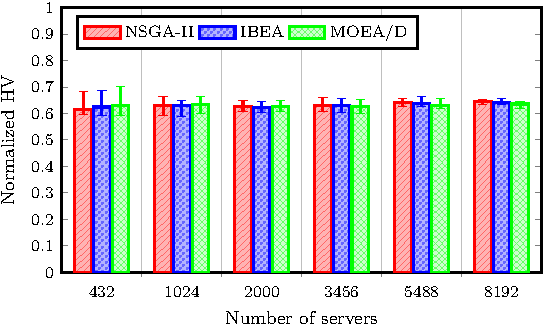
\includegraphics[width=.7\columnwidth]{figs/moeas-crop}
                  \caption{The lower quartile, median, and upper quartile of the hyper-volume of the population for different MOEAs on 30 VNFPP instances.}
                  \label{fig:moea_comparison}
            \end{figure}\\
            \textcolor{blue}{
                  The results of this test are illustrated in~\pref{fig:moea_comparison}. We found that all algorithm performed similarly, with no algorithm performing consistently significantly better than any other. Given all algorithms performed similarly, we have selected NSGA-II for use in future tests based on its widespread adoption in the literature.
                  \textbf{(Page x, highlighted in \textcolor{red}{red} color.)} }

      \item\textsf{My biggest concern is the difference between the proposed method with the author’s previous works. Although the authors tried to illustrate the difference between the proposed algorithm with their previous work [16]. E.g. compared with the proposed work, the work of [16] did not consider the packet loss and is only applicable to small-scale VNFPPs. Could you explain these in detail? E.g. What’s the technique difference between these two works? E.g. Why [16] can only applicable to small-scale VNFPPs? Why the current method can solve the large-scale VNFPPs? }\\
            \textcolor{blue}{\textbf{\textit{Reply}: We thank the reviewer for this comment. There are several key differences between the two algorithms. In our revised manuscript we have elaborated on these distinctions.}}\\
            \textcolor{blue}{\textit{``To the best of our knowledge, our previous work~\cite{TODO} is the only one that combines meta-heuristics with a queueing model for VNFPP. We used a simple solution representation where each solution is represented as a string of VNFs and proposed custom mutation and initialization operators to improve the chances of placing at least one instance of each VNF. It also used a simple queuing model that calculates the latency and energy consumption but does not consider packet loss. In our current work, we propose a more advanced solution representation that allows for more diverse solutions without requiring custom genetic operators. Further, we show that this new representation is simple to extend to complex constraints. Finally, we improve upon the model to consider packet loss and show how this significantly affects the quality of solutions."} \textbf{(Page x, highlighted in \textcolor{red}{red} color.)}}\\

            \textsf{In addition, the authors should compare them in experimental part with the aim to show the advantages of the proposed methods.}\\
            \textcolor{blue}{\textbf{\textit{Reply}: We thank the reviewer for this suggestion. In our revised manuscript we have included our previously proposed algorithm in our comparison.}}\\
            \textcolor{blue}{\textit{``$\cdots$TODO"} \textbf{(Page x, highlighted in \textcolor{red}{red} color.)}}\\

            \textsf{At last, I found that the authors has published a recent work in EMO 2021 named “Parallel Algorithms for the Multiobjective Virtual Network Function Placement Problem”. What’s the main differences between this work and the proposed method? }\\
            \textcolor{blue}{\textbf{\textit{Reply}: We thank the reviewer for this comment. The aforementioned work submitted to EMO and a related work 'Routing-Led Placement of VNFs in Arbitrary Networks' published in WCCI both build upon and reference the paper we are submitting to this journal. Specifically, the WCCI paper explores how this journal paper can be extended to arbitrary networks and the EMO paper applies parallel MOEAs to solve VNFPPs in arbitrary graphs. This journal paper is the keystone work of both of these papers. In particular, both conference papers reference the model, initialization, solution representation and results of this journal paper. Further, although the conference papers above are reliant on this journal paper, they do not restate the concepts introduced in this paper.}}\\

      \item\textsf{In related work part, the sentence “They first pre-processed the network topology to find the most influential nodes according to the Katz centrality.” where the Katz centrality should be followed with a reference.}\\
            \textcolor{blue}{\textbf{\textit{Reply}: We thank the reviewer for identifying this issue and have added a reference to the seminal work \textit{'A new status index derived from sociometric analysis'} by Leo Katz, where the Katz centrality was first proposed.}}\\
            \textcolor{blue}{\textit{``...They first pre-processed the network topology to find the most influential nodes according to the Katz centrality \cite{TODO}."} \textbf{(Page x, highlighted in \textcolor{red}{red} color.)}}\\

      \item\textsf{When the authors presented the proposed Genotype-Phenotype Solution Representation, the authors had better give a illustrated example to show what the solution looks like. Currently, it is somehow abstract.}\\
            \textcolor{blue}{\textbf{\textit{Reply}: We thank the reviewer for this comment. In the updated manuscript we have included a figure illustrating the genotype-phenotype solution representation.}}\\
            \textcolor{blue}{\textbf{(Page x, highlighted in \textcolor{red}{red} color.)}}

      \item\textsf{There are some unclear places when introducing the experimental results. For example, why the Simulation benchmark in Fig. 5 are zero in terms of Latency, Packet Loss and Energy?}\\
            \textcolor{blue}{\textbf{\textit{Reply}: We thank the reviewer for this comment. To clarify, these metrics are only zero when the average arrival rate is zero. This would occur if the data center was not in use.}}\\

            \textsf{What’s the meaning of nodes with different colors in Fig. 6?}\\
            \textcolor{blue}{\textbf{\textit{Reply}: We thank the reviewer for this comment. In these figures, each node represents a solution from the final population. The colours on the figure relate to the latency of each solution but are intended to help the reader to distinguish between solutions. We have improved the caption of each of the relevant figures to better reflect these details, e.g. the caption of Fig. 7 now reads:}}\\
            \textcolor{blue}{\textit{``An illustrative example of the objective values of the solutions found by NSGA-II using our proposed model and
            models from the literature. More diverse solutions with lower objective values indicate more appropriate models."} \textbf{(Page x, highlighted in \textcolor{red}{red} color.)}}

\end{enumerate}

\clearpage


\end{document}
